%----------------------------------------------------------------------------------------
%	CHAPITRE 3
%----------------------------------------------------------------------------------------
\chapter{Procédures de recherches}

\label{Chapter2} % For referencing the chapter elsewhere, use \ref{Chapter2} 

Nous avons définie la notion d'heuristique de recherche, présenté quelques problèmes types rencontrés en y appliquant des heuristiques simples et intuitives ainsi que des contraintes rencontrées lorsque les données à parcourir sont trop importantes et développé différentes méthodes pour modéliser nos problèmes. 
Ce chapitre présente quelques algorithmes et méthodes connus pour parcourir et rechercher des propriétés dans nos graphe (modèle).
Ces algorithmes définissent des stratégies ou politiques de recherche déterminant l'ordre dans lequel les nœuds du graphe seront parcourus afin d'obtenir la solution solution souhaitée ou une solution proche dans le cas d'heuristique.

Dans un premier temps nous présentons les procédures simples avec les algorithmes de parcours de graphe les plus populaires puis nous continuerons sur les recherches avec apprentissage.


%----------------------------------------------------------------------------------------
%	SECTION 1
%----------------------------------------------------------------------------------------
\section{Procédures de recherches simples}
%TODO Petite transition introductif
Nous présentons deux grands types de stratégies que sont les stratégies informées ou à l'aveugle et les stratégies guidées ou informées.

%\subsection{Hill climbing}
%TODO Doit-on faire ce type de parcours ? Il n'est ni informée ni non informée et il faut donc une nouvelle section (P.35)
%La plus populaire. Depuis la position courante, sélectionner la montée la plus rapide.
%Possibilité de trouver un chemin ne finissant jamais et sans solution.
%Comme on ne peut pas passer 2 fois sur un noeud, il faut fermer un chemin si il n'est pas correct et on ne pourra plus le reprendre même pour optimiser son parcours. Il est donc possible de parcourir un chemin à partir de toutes les branches de profondeur 1 sans trouver de solution.

%Avantages: 

%- Quand on connait/possède des informations pour éviter les mauvais parcours et atteindre plus rapidement l'objectif fixé.

%- Histoire sur les expansions commutatives: l'expansion d'un noeud ne compremet pas l'expansion des autres noeuds ou même de leurs descendants. Si une stratégie irrévocable est prise (mauvais chemin) alors cela n'affectera pas les prochains parcours.

\subsection{Recherche non informée}
On dit que la recherche n'est pas informée quand dans un graphe, la location de l'objectif n'altère pas l'ordre dans lequel les nœuds seront parcourus.
Ces stratégies sont souvent inefficaces et peu pratiques dans le cas de larges problèmes mais elles ont l'avantages d'être simples et peuvent être appliquées à tout problème puisqu'elles ne prennent  pas compte des données propres au domaine.

\subsubsection{Parcours en profondeur (DFS)}
Le parcours en profondeur donne la priorité aux nœuds les plus profonds du graphe et s'applique plus particulièrement au graphe de type arbre ou la profondeur est clairement définie.
Pour les autres types de graphe, il faudra définir la notion de profondeur et la direction dans laquelle se diriger.

Ce type de parcours assure de trouver la solution, puisqu'en pire cas toutes les solutions seront énumérées ce qui rend cet algorithme peu efficace dans de nombreux cas.\\
%TODO lesquels ?

%Variante backtracking
{\setlength{\parindent}{0cm}\textbf{backtracking:}}

Le \textit{backtracking} (ou retour sur trace) est une variante du parcours en profondeur qui permet de revenir en arrière à chaque action afin de minimiser le nombre de sommets du graphe à parcourir quand on se retrouve dans certaines situations qui ne correspondent pas à l'objectif recherché (propriétés d'un nœud non conforme).

%TODO
% C'est une version du parcours en profondeur qui applique la politique de dernier-entrée-premier-sortie (LIFO) pour la génération des nœuds au lieu de l'expansion.

A chaque nœud, seulement un successeur est parcouru sauf si il ne remplit pas un critère donné. Dans le cas où il ne serait pas parcouru on revient à l'ancêtre le plus proche parcouru possédant au moins 1 sommet fils qui n'a pas été encore parcouru.

\begin{center}
    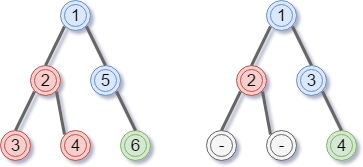
\includegraphics[scale=0.6]{../ressources/images/depth_first_search.png}
    \captionof{figure}{Ordre dans lequel les sommets sont visités avec un parcours en profondeur (gauche) et sa variante (droite): le backtracking.}
\end{center}

Les problèmes d'optimisation ou de semi-optimisation tire parti de ce type de parcours. Si l'objectif est de trouver le coût minimal alors cette stratégie est efficace puisqu'elle permet de parcourir le graphe tout en maintenant le coût à tout instant t et ceci en priorisant les sommets les plus proches de la racine.

\subsubsection{Parcours en largeur (BFS)}
Contrairement au parcours en profondeur, le parcours en largeur donne la priorité au nœuds des premiers niveaux du graphe, c'est à dire aux sommets les plus proches de la racine qui seront parcourus en premier. Elle s'applique plus facilement aux arbres puisque la notion de niveau est naturellement défini, contrairement aux autres types de graphe ou il faudra définir ce qu'on entend par largeur pour orienter le sens du parcours.

Cette stratégie garantie aussi de trouver la meilleure solution possible puisque en pire cas, tout le graphe sera parcouru. C'est donc une méthode qui peut rapidement devenir très couteuse.\\

%Variante procédure du coût uniforme
{\setlength{\parindent}{0cm}\textbf{Procédure du coût uniforme:}}

La procédure du coût une uniforme est une variante du parcours en largeur. Au lieu de procéder au parcours des nœuds d'une même profondeur, le parcours se fait en fonction du coût des nœuds. Chaque nœud est exprimé comme étant le coût du chemin menant à lui depuis le nœud racine et la stratégie est accomplie en parcourant toujours le nœud avec le coût le plus faible.

\begin{center}
    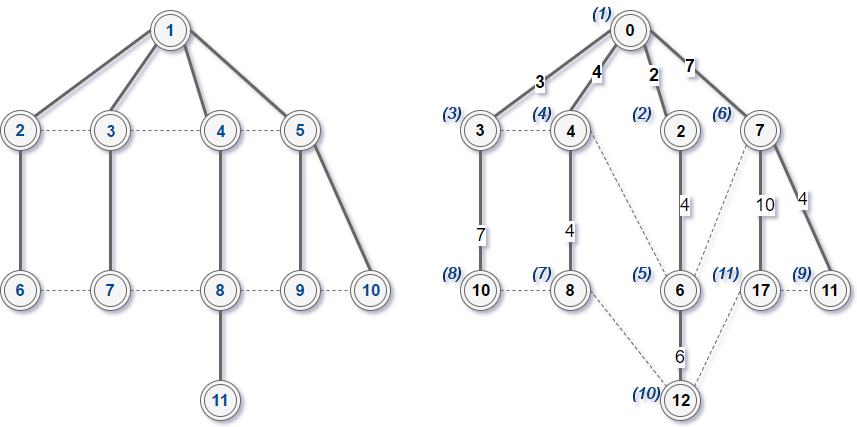
\includegraphics[scale=0.5]{../ressources/images/breath_first_search.png}
    \captionof{figure}{Ordre dans lequel les sommets sont visités avec un parcours en largeur (gauche) et sa variante (droite): la procédure du coût uniforme.}
\end{center}

\subsection{Recherche informée}
Nous avons vu précédemment des stratégies qui ne prenaient pas en compte les données du problème autre que celles définies dans les sommets et les arêtes. Parfois il est possible de tirer parti d'informations qui ne sont pas dans le graphe pour diriger les recherches afin de parcourir les sommets qui ont l'air d'être les plus prometteurs.
Cette section présente l'intérêt de combiner des méthodes (fonctions) heuristiques aux parcours classiques.

\subsubsection{Best-First search (le meilleur d'abord)}
\textit{Best-first search} est un algorithme qui parcourt le graphe en étendant le nœud le plus prometteur d'abord. Contrairement aux heuristiques gloutonnes qui elles aussi sélectionnent les meilleurs éléments d'abord, \textit{best-first search} le fait par évaluation, c'est à dire en estimant la valeur d'un nœud avant de le parcourir à partir de données du problème qui ne sont pas présent dans le graphe, comme une fonction heuristique qui permet d'estimer la valeur d'un nœud (récompense). De plus l'objectif de cette méthode n'est pas seulement de sélectionner le sommet le plus prometteur parmi un ensemble de nœud à prochainement parcourir mais de le sélectionner en comparant tous les sommets déjà rencontrés.

La promesse, c'est à dire l'estimation de la qualité d'un nœud est estimé grâce à une fonction heuristique $f(n)$ qui peut dépendre des données du sommet $n$, de la description de l'objectif recherché, des informations récoltées lors du parcours de recherche et de toutes informations supplémentaires sur le domaine.\\

%TODO Définir fonction heuristique d'évaluation

%TODO Présenter l'algorithme

%TODO Montrer l'algorithme tel qu'il est présent dans le livre

\textbf{L'algorithme best-first décrit par Judea pearl\cite{judea-pearl-heuristics}}
\begin{enumerate}
\item Mettre le nœud racine (initial) dans la liste $NOEUDS OUVERTS$.
\item Si la liste $NOEUDS OUVERTS$ est vide, arrêter le programme: pas de solution.
\item Déplacer le nœud le plus prometteur de $NOEUDS OUVERTS$ c'est à dire celui pour lequel la fonction heuristique \textit{f} est minimum (ou maximum dans un problème de maximisation) dans la liste $NOEUDS FERMES$. On nomme ce nœud $n$.
\item Si l'un des successeurs de $n$ est l'objectif alors retourné le chemin vers ce nœud.
\item Pour chacun des successeurs $n'$ de n:
    \begin{enumerate}
    \item Calculer $f(n')$.
    \item Si $n'$ n'était ni dans la liste $NOEUDS OUVERTS$ ni $NOEUDS FERMES$, l'ajouter dans la liste $NOEUDS OUVERTS$. Attaché l'évaluation de l'heuristique au nœud ainsi qu'un lien vers le nœud $n$.
    \item Sinon comparer le résultât de la fonction heuristique avec le résultât enregistré (qui a été précédemment attaché au nœud). Si l'ancienne évaluation est meilleure (inférieure ou supérieure selon le problème de minimisation ou maximisation) alors passer à l'étape suivante. Si l'ancienne évaluation est moins bonne, remplacer l'évaluation ainsi que le lien  pour pointer vers le nœud $n$. Si le nœud $n$ est dans la liste $NOEUDS FERMES$, le déplacer dans $NOEUDS OUVERTS$.
    \end{enumerate}
\item Retourner à l'étape 2.
\end{enumerate}

%TODO Conclure sur l'intérêt de Best-first, pourquoi on l'utilise ? (P.49)
%TODO Définir clairement la différence avec la procédure du coût uniforme.

\subsubsection{Algorithmes best-first spécialisés}
Pour explorer un minimum de sommets possibles dans un graphe à la recherche d'un chemin optimal, un algorithme de recherche doit constamment faire les choix les plus informés possibles pour décider du prochain prochain nœud à explorer.

L'algorithme \textit{best-first search} n'est que la patron d'une stratégie à appliquer et nécessite d'être plus amplement définie pour être implémenté concrètement.
Il ne spécifie pas comment la fonction heuristique $f$ est calculé ni d'où les informations pour décider quel est le meilleur choix possible proviennent ou même comment elles se propagent sur le graphe pourtant se sont les éléments indispensables à une recherche efficace. \\

{\setlength{\parindent}{0cm}\textbf{A*:}}

L'algorithme \textit{A*} est un algorithme de type \textit{best first} et est aussi une extension de l'algorithme de Dijkstra\cite{dijkstra} un des plus populaires pour résoudre le problème du plus court chemin. 

L'algorithme A* définie\cite{description-a*} sa fonction d'évaluation comme suivant: 

\begin{center}
    $f(n) = g(n) + h(n)$
\end{center}

où $g(n)$ est le coût d'un chemin optimal du sommet racine $s$ vers le sommet $n$ et où $h(n)$ est le coût d'un chemin optimal du sommet $n$ vers le sommet $a$, un éventuel nœud objectif.\\    

%TODO Compléter les informations sur A* et donner un exemple où il est utile

\textbf{L'algorithme A*\cite{description-a*}}
\begin{enumerate}
\item Mettre le nœud racine (initial) dans la liste $NOEUDS OUVERTS$.
\item Si la liste $NOEUDS OUVERTS$ est vide, arrêter le programme: pas de solution.
\item Déplacer le nœud le plus prometteur de $NOEUDS OUVERTS$ c'est à dire celui pour lequel la fonction heuristique \textit{f} est minimum dans la liste $NOEUDS FERMES$. On nomme ce nœud $n$.
\item Si $n$ est l'objectif alors retourné le chemin vers ce nœud.
\item  Pour chacun des successeurs $n'$ de n:
    \begin{enumerate}
    \item Si $n'$ n'est pas dans $NOEUDS OUVERTS$ ou $NOEUDS FERMES$, estimé $h(n')$ (une estimation du coût du meilleur chemin de $n'$ vers un éventuel nœud objectif) et calculer $f(n') = g(n') + h(n')$ où $g(n') = g(n) + c(n, n')$ and $g(s) = 0$ où s est le nœud racine.
    \item Si $n'$ est dans $NOEUDS OUVERTS$ ou  $NOEUDS FERMES$. 
    \item Si $n'$ la condition de l'étape précédente est vraie et que $n'$ est dans la liste de $NOEUDS FERMES$ alors déplacer $n'$ dans $NOEUDS OUVERTS$.
    \end{enumerate}
\item Retourner à l'étape 2. 
\end{enumerate}

%TODO Conclusion + transition

%----------------------------------------------------------------------------------------
%	SECTION 3
%----------------------------------------------------------------------------------------

\section{Procédures de recherches avec apprentissage}
%TODO C'est quoi l'apprentissage 
L'apprentissage automatique est un champs d'étude de l'intelligence artificielle.
Appliquée à certaines méthodes systématiques elle permet d'exécuter des tâches complexes en mémorisant des informations obtenues lors de chaque étape. Il est par exemple possible d'utiliser cette méthode pour classifier, c'est à dire qu'on étiquette chaque donnée rencontrée en fonction de ses propriétés à des fins de regroupement ou de génération de nouvelles connaissances pouvant faciliter le traitement par des méthodes automatiques. 
%TODO Pourquoi appliquer des mécaniques d'apprentissage à nos problèmes ?

\subsection{Monte Carlo Tree Search (MCTS)}

\subsubsection*{Définitions}
\textit{Monte Carlo Tree Search} (MCTS) est avant tout une méthode pour la résolution pratique de jeux, son application permet de décider des prochaines actions (optimales) à jouer à partir du résultât de simulation faites sur des parties fictives et des actions effectuées par l'adversaire.
Le processus du MCTS est le suivant: un arbre est construit de manière incrémental et asynchrone et pour chaque itération de l'algorithme, une politique est utilisée pour déterminer quel est le prochain nœud à parcourir depuis l'état actuel. Cette politique est appelée, politique de l'arbre et son rôle est d'équilibrer l'exploration de nouveaux nœuds (parcourir de nouveaux nœuds) et l'exploitation des nœuds déjà parcouru pour maximiser les informations récoltées jusqu'à alors. Puis une simulation est effectuée depuis le dernier nœud sélectionné pour évaluer sa distance avec l'objectif cherché (a t-on des chances d'atteindre l'objectif et en combien de coup pouvons nous l'atteindre ?). Ensuite, grâce au résultât de cette évaluation, tous les nœuds parcourus jusqu'à alors pour atteindre le nœud actuellement sélectionné sont mis à jour pour tenir compte du résultât de la simulation. Les nœuds parcourus contiennent donc des statistiques qui permettent d'évaluer leur potentiel.

\begin{center}
    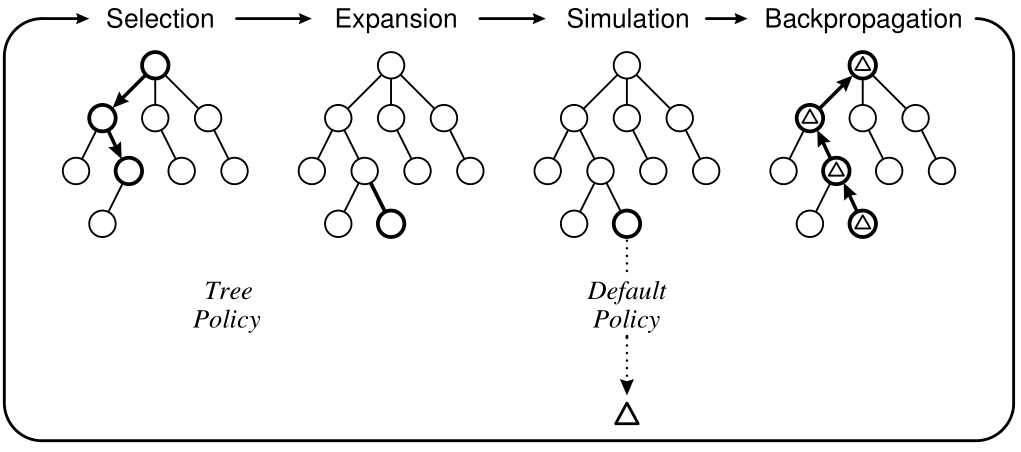
\includegraphics[scale=0.5]{../ressources/images/MCTS-example-iteration.png}
    \captionof{figure}{Une itération du MCTS - source: \textit{A Survey of Monte Carlo Tree Search Methods}\cite{MCTS-methods-survey}}
    \label{example-mcts-iteration}
\end{center}

Les performances de MCTS dépendent donc du nombre de simulations produites puisqu'elles permettent à la recherche de s'orienter automatiquement vers les coup les plus prometteurs en fonction des données récoltées lors des simulations. MCTS appartient à la famille des méthodes d'apprentissage par renforcement puisque les répétitions des itérations successives permettront à l'algorithme d'affiner ses connaissances du problème.
Même si l'algorithme de base du MCTS s'est prouvé intéressant et efficace, le vrai bénéfice d'utiliser de MCTS est atteint lorsque l'algorithme est adapté au problème donné. Les variantes du MCTS sont donc tout aussi intéressantes et il est important d'adapter le comportement général de MCTS face à chaque situation.


\subsection*{Limitations}
Il faut être en mesure de simuler les résultats possibles depuis un nœud. Il faut donc être capable de connaître les actions qui peuvent être entreprises depuis le contexte actuel et c'est pour cette raison que cette méthode a eu un tel succès pour la résolution pratique de jeux. De plus, cette simulation fait l'objet de nombreuses recherche puisqu'elle 


%Un des avantages de MCTS est que sa fonction d'évaluation n'a pas besoin d'être définie, elle est ajustée dynamiquement à partir du résultât des évaluations.
%Depuis les 

%Inconvénients:
%Les performances de MCTS dépendent du nombre de simulations que l'oracle est capable de réaliser à chaque itération.

%Algorithme:
%Un arbre est construit de manière incrémental et asynchrone. Pour chaque itération de l'algorithme, une politique est utilisée pour trouver le noeud le plus important de l'arbre actuel.
%La politique d'arbre essaie d'équilibrer entre l'exploration de l'arbre (regarder dans les zones qui n'ont pas été essayées) et l'exploitation (regarder dans les zones qui ont l'air prometteuses).
%
%Depuis un nœud une simulation est lancée et l'arbre se met à jour en fonction du résultât. Cela implique l'apparition d'un nœud correspondant à l'action entreprise par l'algorithme.
%
%Les mouvements sont effectués pendant la simulation selon une politique d'arbre pré-défini par défaut qui dans le plus simple des cas consiste à effectuer des mouvements aléatoires uniforme.

%MCTS n'a besoin que de l'état terminal de la simulation précédente pour effectuer la suivante. Il n'utilise pas les états intermédiaires.
%L'avantage est que cela réduit grandement les connaissances nécessaires à l'exécution de la méthode.
%
%Même si l'algorithme est efficace sur une grande variété de problème, le vrai bénéfice d'utiliser MCTS est lorsqu'il est adapté au domaine du problème.
%
%Méthode Monte-Carlo:
%%(Différent de MCTS)
%Évaluation de la récompense: 
%
%$Q(s, a) = 1 / N(s, a)$ ... % (P.2)
%
%\subsubsection*{Variantes}
%%TODO
%Deux concepts fondamentaux:
%
%- La valeur réelle d'une action peut être approchée en utilisant une simulation aléatoire.
%
%- Ces valeurs peuvent être utilisées pour ajuster la politique vers une stratégie du meilleur d'abord (Best-First).
%
%L'algorithme construit progressivement un arbre de décision guidé par les résultâts des explorations précédentes.
%L'arbre est utilisé pour estimer les valeurs associées à chaque mouvement.
%
%Algorithme: 
%
%Basique: Construction itérative d'un arbre de recherche jusqu'à ce qu'un critère prédéfini soit atteint. Souvent une limite de de calcul comme le temps d'exécution, ou la saturation de la mémoire.
%%TODO (P.6 Fig 2. Schéma de l'algorithme, surement à mettre dans le mémoire.
%
%1. Sélection: depuis le noeud racine, une politique est appliquée pour sélectionner les noeuds pour atteindre le noeud le plus important à étendre (noeud non visité et non terminal).
%
%2. Expansion: Un ou plusieurs noeuds son ajoutés pour étendre l'arbre (choix en fonction des actions disponibles).
%
%3. Simulation: une simulation est appliquée depuis le nouveau noeud en fonction d'une politique par défaut pour produire un résultât.
%
%4. Backpropagation: Le résultât de la simulation est remotée à travers les noeuds sélectionnés pour arriver au noeud ajouté pour mettre à jour ses statistiques.
%
%Deux politiques: 
%
%- La politique de l'arbre: sélectionner ou créer un noeud feuille depuis les noeuds déjà parcourus/ajoutés.
%
%- La politique par défaut: estimer la valeur d'un état non terminal (noeud ajouté) pour produire une estimation de sa valeur.

%\subsubsection*{Applications}

%TODO Montrer les cas d'applications les plus populaires comme pour le jeu de GO.

%TODO Montrer d'autres cas d'applications
%Des applications pour des problèmes du plus court chemin (problème du voyageur). Il est efficace pour le problème du voyageur canadien où certain des chemins peuvent être bloqués avec une certaine probabilité (utilisation d'une variante UCT).

%\subsection{Forêt d'arbres décisionnels (random forest)}
%Random forest une technique ensemblistes pour l'analyse 
%
%
%\subsection{Algorithme de programmation génétique}

%\subsection{Théorie de la décision}
%TODO
%Elle combine les théories probabilistiques avec des théories utilitaires (heuristiques) pour offrir une approche formelle pour la prise de décision dans l'incertain.

%Processus de décision Markovien: Modélise de manière séquentielle des problèmes de décision dans un environnement entièrement observable.
%Les décisions sont modélisées comme un ensemble d'état, action dans lequel chacun des prochains états est évalués grâce à une distribution de probabilité en fonction de l'état courant et de l'action entreprise.
%Une politique est une correspondance entre états et actions en spécifiant quel action doit être entreprise depuis chaque état.
%L'objectif et de déterminer la politique qui permette de maximiser la récompose.
%La fonction de transition évalue la probabilité depuis l'état s et l'action a de se retrouver dans l'état s' (les états sont incertains).


%Processus de décision Markovien partiellement  observable (POMDP):
%Contrairement à l'approche MDP, l'oracle n'a qu'une information partielle de l'état courant.

%\subsection{Les autres procédures}
